% ============================================================
%  Saudi Location Intelligence MCP Server --- Technical Documentation
% ============================================================
\documentclass[12pt,a4paper]{report}

% --- Encoding & fonts ---
\usepackage[T1]{fontenc}
\usepackage[utf8]{inputenc}
\usepackage{lmodern}
\usepackage{microtype}

% --- Page geometry ---
\usepackage[top=2.5cm, bottom=2.5cm, left=2.8cm, right=2.8cm]{geometry}

% --- Colours ---
\usepackage{xcolor}
\definecolor{codebg}{HTML}{F5F5F5}
\definecolor{accent}{HTML}{1A5276}
\definecolor{lightaccent}{HTML}{D6EAF8}
\definecolor{filecolor}{HTML}{117A65}
\definecolor{warningbg}{HTML}{FEF9E7}

% --- Graphics ---
\usepackage{graphicx}
\graphicspath{{figures/}}

% --- Code listings ---
\usepackage{listings}
\lstset{
  backgroundcolor=\color{codebg},
  basicstyle=\ttfamily\small,
  breaklines=true,
  breakatwhitespace=true,
  frame=single,
  rulecolor=\color{gray!40},
  keywordstyle=\color{blue!70!black}\bfseries,
  commentstyle=\color{green!50!black}\itshape,
  stringstyle=\color{red!60!black},
  showstringspaces=false,
  tabsize=4,
  captionpos=b,
  numbers=left,
  numberstyle=\tiny\color{gray},
  numbersep=6pt,
}
\lstdefinelanguage{mermaid}{
  keywords={graph,flowchart,sequenceDiagram,TD,LR,RL},
  sensitive=false,
  comment=[l]{\%\%},
  morestring=[b]",
}

% --- Tables ---
\usepackage{booktabs}
\usepackage{longtable}
\usepackage{array}
\usepackage{tabularx}

% --- Boxes / callouts ---
\usepackage{mdframed}
\mdfdefinestyle{filebox}{
  backgroundcolor=lightaccent,
  linecolor=accent,
  linewidth=1.5pt,
  innerleftmargin=10pt,
  innerrightmargin=10pt,
  innertopmargin=6pt,
  innerbottommargin=6pt,
  roundcorner=4pt,
}
\mdfdefinestyle{notebox}{
  backgroundcolor=warningbg,
  linecolor=orange!70!black,
  linewidth=1pt,
  innerleftmargin=10pt,
  innerrightmargin=10pt,
  innertopmargin=6pt,
  innerbottommargin=6pt,
}

% --- Section formatting ---
\usepackage{titlesec}
\titleformat{\chapter}[display]
  {\normalfont\Large\bfseries\color{accent}}
  {Chapter \thechapter}{12pt}{\Huge}
\titleformat{\section}
  {\normalfont\large\bfseries\color{accent}}
  {\thesection}{1em}{}
\titleformat{\subsection}
  {\normalfont\normalsize\bfseries\color{filecolor}}
  {\thesubsection}{1em}{}

% --- Header/Footer ---
\usepackage{fancyhdr}
\pagestyle{fancy}
\fancyhf{}
\fancyhead[L]{\small\textcolor{gray}{Saudi Location Intelligence MCP Server}}
\fancyhead[R]{\small\textcolor{gray}{\leftmark}}
\fancyfoot[C]{\small\thepage}
\renewcommand{\headrulewidth}{0.4pt}

% --- Hyperlinks ---
\usepackage[colorlinks=true, linkcolor=accent, urlcolor=blue!70!black, citecolor=green!50!black]{hyperref}

% --- Misc ---
\usepackage{enumitem}
\usepackage{float}
\usepackage{caption}
\captionsetup{font=small, labelfont=bf}
\setlength{\parskip}{4pt}

% ============================================================
\begin{document}

% ---- Title Page ----
\begin{titlepage}
  \centering
  \vspace*{3cm}
  {\color{accent}\rule{\linewidth}{1.5pt}}\\[1.5em]
  {\Huge\bfseries\color{accent} Saudi Location Intelligence\\[0.4em] MCP Server}\\[1em]
  {\Large Technical Documentation}\\[0.5em]
  {\color{accent}\rule{\linewidth}{1.5pt}}\\[3em]
  {\large\textit{Complete codebase walkthrough with architecture diagrams,\\
  data flow charts, and module-level explanations}}\\[5cm]
  {\large Version 1.0.0}\\[0.5em]
  {\large\today}
  \vfill
\end{titlepage}

\tableofcontents
\listoffigures
\newpage

% ============================================================
\chapter{Project Overview}
% ============================================================

\section{What Is This Project?}

The \textbf{Saudi Location Intelligence MCP Server} is a server built on the
\href{https://modelcontextprotocol.io}{Model Context Protocol (MCP)} that exposes
geospatial analysis tools to AI clients (such as Claude) or developer tools such
as the MCP Inspector.

It acts as a \emph{bridge} between an AI model and a backend REST API that holds
Saudi Arabia location data --- points of interest, real estate, demographics,
and business analytics. The AI client calls a \emph{tool} (e.g.\ \texttt{fetch\_geospatial\_data}),
the MCP server authenticates the request, proxies it to the backend, stores the
result on disk, and returns a lightweight \emph{handle} plus a human-readable
summary back to the AI.

\section{Key Capabilities}

\begin{itemize}[noitemsep]
  \item \textbf{Geospatial data fetching} --- POI, real estate, demographics for Saudi cities
  \item \textbf{Territory optimisation} --- spatial clustering for sales-team planning
  \item \textbf{Hub expansion analysis} --- multi-criteria site scoring with AI reports
  \item \textbf{Pharmacy site selection} --- weighted scoring across traffic, competition, demographics
  \item \textbf{Academic \& executive report generation} --- markdown reports with statistical analysis
  \item \textbf{LLM-powered report analysis} --- Gemini-backed natural language Q\&A over reports
  \item \textbf{Session management} --- JWT authentication with automatic token refresh
\end{itemize}

\section{Technology Stack}

\begin{center}
\begin{tabularx}{\linewidth}{lX}
  \toprule
  \textbf{Layer} & \textbf{Technology} \\
  \midrule
  Protocol & Model Context Protocol (MCP) via \texttt{mcp[cli]} \\
  Web framework & Starlette / uvicorn (SSE transport) \\
  Data validation & Pydantic v2 \\
  HTTP client & aiohttp (async) \\
  File I/O & aiofiles + custom file-locking \\
  AI analysis & LangChain + Google Gemini \\
  Runtime & Python 3.13 \\
  Container & Docker (python:3.13-slim + uv) \\
  Build & tectonic (this document) \\
  \bottomrule
\end{tabularx}
\end{center}

\section{High-Level Architecture}

Figure~\ref{fig:architecture} shows all major components and how they connect.

\begin{figure}[H]
  \centering
  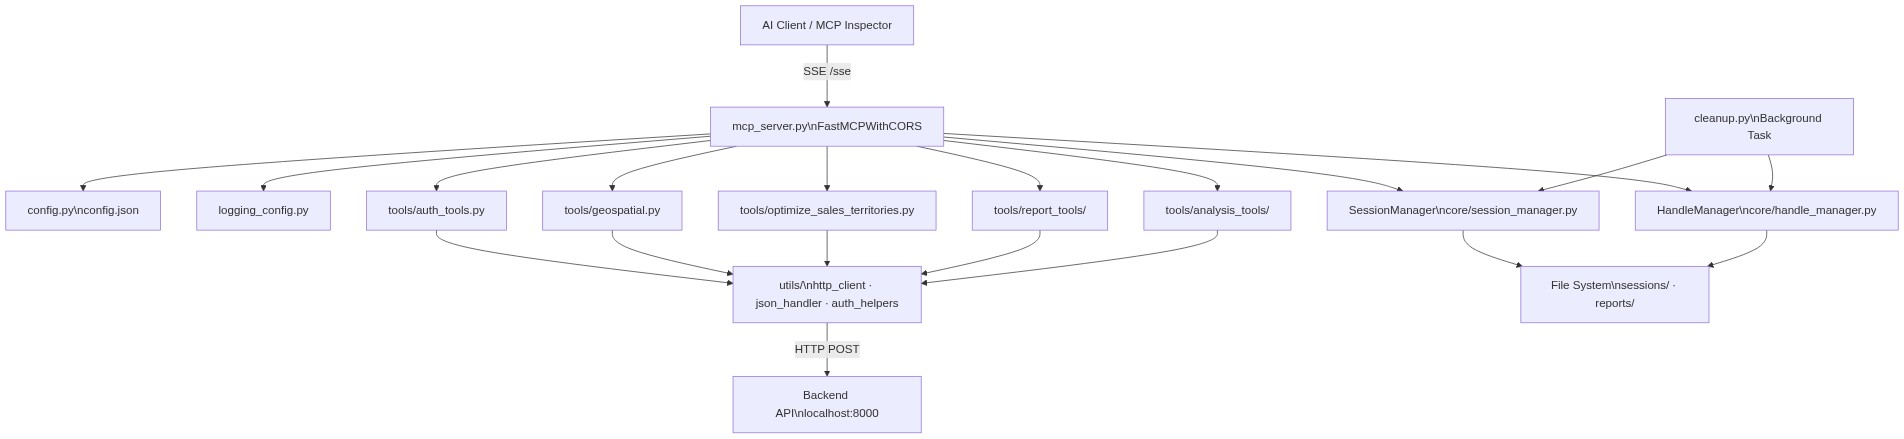
\includegraphics[width=\linewidth]{01_architecture_overview.png}
  \caption{High-level system architecture}
  \label{fig:architecture}
\end{figure}

The server starts as a single Python process. An AI client connects over
\textbf{SSE} (Server-Sent Events) to \texttt{/sse}. The MCP layer routes
each tool call to the registered handler, which uses shared \texttt{SessionManager}
and \texttt{HandleManager} singletons, calls the backend over HTTP, and writes
results to disk.

% ============================================================
\chapter{Configuration Layer}
% ============================================================

\section{\texttt{config.json} --- Runtime Configuration File}

\begin{mdframed}[style=filebox]
\textbf{File:} \texttt{config.json} \hfill \textbf{Format:} JSON
\end{mdframed}

\texttt{config.json} lives at the project root and provides defaults that can
be overridden at runtime by environment variables (important for Docker
deployments):

\begin{lstlisting}[language={},caption={Typical config.json}]
{
  "backend_url":             "http://localhost:8000",
  "server_host":             "0.0.0.0",
  "server_port":             8001,
  "cors_origins":            "*",
  "session_ttl_hours":       8,
  "cleanup_interval_hours":  1,
  "sessions_path":           "sessions",
  "reports_path":            "reports"
}
\end{lstlisting}

\section{\texttt{config.py} --- Configuration Module}

\begin{mdframed}[style=filebox]
\textbf{File:} \texttt{config.py} \hfill \textbf{Imports used by:} every module
\end{mdframed}

\subsection{Responsibility}

\texttt{config.py} is the \emph{single source of truth} for all configuration.
It loads \texttt{config.json} once at import time, then checks environment
variables and lets them override the JSON values. Every other module imports
constants from here --- no module reads environment variables directly.

\subsection{Loading Flow}

\begin{figure}[H]
  \centering
  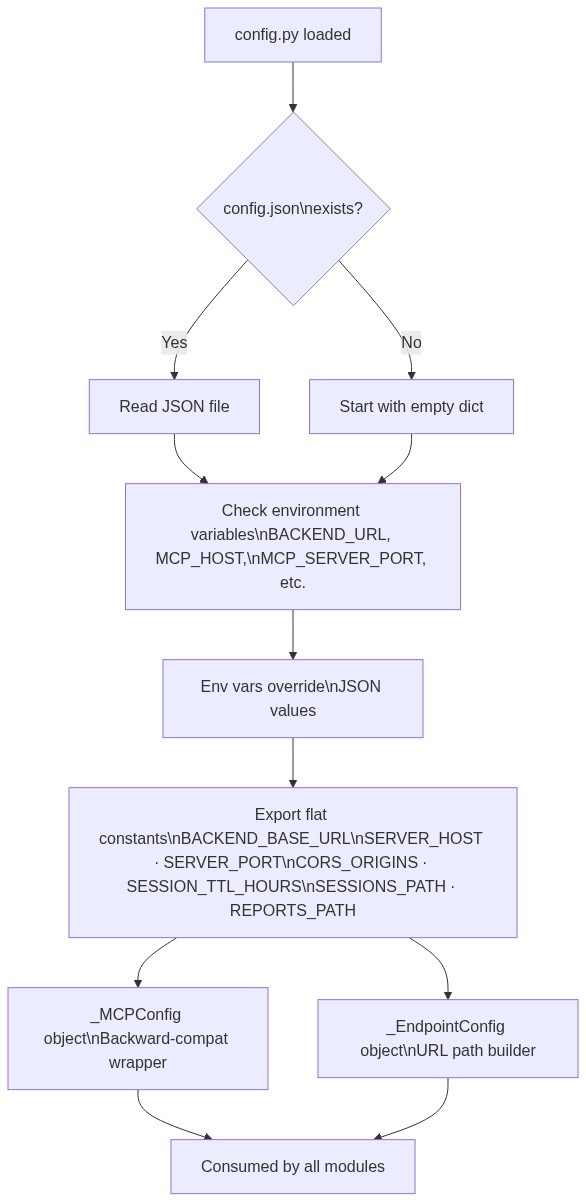
\includegraphics[width=0.85\linewidth]{02_config_flow.png}
  \caption{Configuration loading sequence}
  \label{fig:config}
\end{figure}

\subsection{Exported Constants}

\begin{center}
\begin{tabularx}{\linewidth}{llX}
  \toprule
  \textbf{Constant} & \textbf{Env Override} & \textbf{Purpose} \\
  \midrule
  \texttt{BACKEND\_BASE\_URL} & \texttt{BACKEND\_URL} & URL of the backend REST API \\
  \texttt{SERVER\_HOST}       & \texttt{MCP\_HOST} & Bind address for uvicorn \\
  \texttt{SERVER\_PORT}       & \texttt{MCP\_SERVER\_PORT} & Port for uvicorn \\
  \texttt{CORS\_ORIGINS}      & \texttt{CORS\_ORIGINS} & Comma-separated allowed origins \\
  \texttt{SESSION\_TTL\_HOURS} & \texttt{SESSION\_TTL\_HOURS} & Session expiry window \\
  \texttt{CLEANUP\_INTERVAL\_HOURS} & \texttt{CLEANUP\_INTERVAL\_HOURS} & Background cleanup cadence \\
  \texttt{SESSIONS\_PATH}     & --- & Absolute path to sessions directory \\
  \texttt{REPORTS\_PATH}      & --- & Absolute path to reports directory \\
  \bottomrule
\end{tabularx}
\end{center}

\subsection{Backward-Compatible Wrappers}

Two small classes wrap the flat constants so that existing call-sites that
accessed \texttt{config.session\_ttl\_hours} or \texttt{ENDPOINTS.login}
continue to work without changes:

\begin{itemize}[noitemsep]
  \item \textbf{\texttt{\_MCPConfig}} (\texttt{config} instance) --- exposes \texttt{session\_ttl\_hours}, \texttt{cleanup\_interval\_hours}, \texttt{temp\_storage\_path}
  \item \textbf{\texttt{\_EndpointConfig}} (\texttt{ENDPOINTS} instance) --- builds full endpoint paths by prepending \texttt{/fastapi/} to route names (\texttt{.login}, \texttt{.fetch\_dataset}, etc.)
\end{itemize}

% ============================================================
\chapter{Logging}
% ============================================================

\section{\texttt{logging\_config.py} --- Structured Logging}

\begin{mdframed}[style=filebox]
\textbf{File:} \texttt{logging\_config.py}
\end{mdframed}

\subsection{Responsibility}

Provides a consistent, structured logging setup with two output channels:
\begin{itemize}[noitemsep]
  \item \textbf{stderr} --- always visible in the terminal / Docker logs
  \item \textbf{Log files} --- one file per session stored in \texttt{sessions/<id>/session.log}
\end{itemize}

\subsection{Key Functions}

\begin{center}
\begin{tabularx}{\linewidth}{lX}
  \toprule
  \textbf{Function} & \textbf{Description} \\
  \midrule
  \texttt{setup\_main\_logging()} & Called once at startup; attaches stderr + file handler to the root logger \\
  \texttt{get\_logger(name)} & Returns a \texttt{logging.Logger}; ensures main logging is initialised first \\
  \texttt{setup\_session\_logging(session\_id)} & Creates a session-scoped file handler; all tool log output goes here \\
  \texttt{end\_session\_logging(session\_id)} & Flushes and removes the session handler when the session ends \\
  \bottomrule
\end{tabularx}
\end{center}

\begin{mdframed}[style=notebox]
\textbf{Note:} Every module calls \texttt{get\_logger(\_\_name\_\_)} at module level,
so log messages always carry the originating module's name for easy filtering.
\end{mdframed}

% ============================================================
\chapter{Data Models}
% ============================================================

\section{\texttt{models.py} --- Core Pydantic Models}

\begin{mdframed}[style=filebox]
\textbf{File:} \texttt{models.py}
\end{mdframed}

Two Pydantic models represent runtime state persisted to disk as JSON:

\subsection{\texttt{DataHandle}}

Metadata for a single stored data file. Fields:

\begin{center}
\begin{tabularx}{\linewidth}{llX}
  \toprule
  \textbf{Field} & \textbf{Type} & \textbf{Meaning} \\
  \midrule
  \texttt{session\_id}  & \texttt{str}      & Which session owns this data \\
  \texttt{data\_type}   & \texttt{str}      & Category: \texttt{geospatial\_data}, \texttt{hub\_analysis}, etc. \\
  \texttt{location}     & \texttt{str}      & City or region slug \\
  \texttt{expires\_at}  & \texttt{datetime} & When this handle expires \\
  \texttt{file\_path}   & \texttt{str}      & Absolute path to the JSON file on disk \\
  \texttt{summary}      & \texttt{dict}     & Human-readable summary metadata \\
  \texttt{schema}       & \texttt{dict}     & Optional schema description \\
  \bottomrule
\end{tabularx}
\end{center}

\subsection{\texttt{SessionInfo}}

Represents a user session. Fields:

\begin{center}
\begin{tabularx}{\linewidth}{llX}
  \toprule
  \textbf{Field} & \textbf{Type} & \textbf{Meaning} \\
  \midrule
  \texttt{session\_id}       & \texttt{str}           & UUID for this session \\
  \texttt{created\_at}       & \texttt{datetime}      & Creation timestamp \\
  \texttt{expires\_at}       & \texttt{datetime}      & Expiry timestamp \\
  \texttt{data\_handles}     & \texttt{list[str]}     & Filenames of stored data blobs \\
  \texttt{user\_id}          & \texttt{str | None}    & Authenticated user ID \\
  \texttt{id\_token}         & \texttt{str | None}    & JWT ID token \\
  \texttt{refresh\_token}    & \texttt{str | None}    & JWT refresh token \\
  \texttt{token\_expires\_at} & \texttt{datetime | None} & When the ID token expires \\
  \bottomrule
\end{tabularx}
\end{center}

\section{\texttt{all\_types/request\_dtypes.py} --- API Request Models}

\begin{mdframed}[style=filebox]
\textbf{File:} \texttt{all\_types/request\_dtypes.py}
\end{mdframed}

Pydantic models that mirror the backend API's expected request bodies.
They are built by the tool functions and serialised with \texttt{.model\_dump()}
before being sent over HTTP.

\begin{center}
\begin{tabularx}{\linewidth}{lX}
  \toprule
  \textbf{Model} & \textbf{Purpose} \\
  \midrule
  \texttt{Coordinate} & lat/lng pair \\
  \texttt{ReqCityCountry} & city\_name + country\_name \\
  \texttt{UserId} & user\_id string \\
  \texttt{BooleanQuery} & boolean\_query search string \\
  \texttt{ReqFetchDataset} & Full geospatial fetch request (inherits Coordinate + ReqCityCountry) \\
  \texttt{ReqClustersForSalesManData} & Territory clustering request (inherits BooleanQuery + UserId + ReqCityCountry) \\
  \bottomrule
\end{tabularx}
\end{center}

% ============================================================
\chapter{Application Context}
% ============================================================

\section{\texttt{context.py} --- Dependency Injection Helper}

\begin{mdframed}[style=filebox]
\textbf{File:} \texttt{context.py}
\end{mdframed}

\subsection{Problem Solved}

Tool functions are defined inside \texttt{register\_*(mcp)} functions.
They need access to the global \texttt{session\_manager} and \texttt{handle\_manager}
singletons created in \texttt{mcp\_server.py}. Importing them directly would create
circular imports.

\subsection{Solution}

\texttt{context.py} defines \texttt{AppContext} (a \texttt{@dataclass}) and
a helper \texttt{get\_app\_context(mcp)} that imports the singletons \emph{lazily}
at call time:

\begin{lstlisting}[language=Python, caption={get\_app\_context helper}]
def get_app_context(mcp: "FastMCP") -> AppContext:
    from mcp_server import session_manager, handle_manager
    return AppContext(
        session_manager=session_manager,
        handle_manager=handle_manager,
    )
\end{lstlisting}

Every tool calls \texttt{get\_app\_context(mcp)} at the top of its body, giving it
fully typed access to both managers without any import-time circular dependency.

% ============================================================
\chapter{Core Modules}
% ============================================================

\section{\texttt{core/session\_manager.py} --- Session Lifecycle}

\begin{mdframed}[style=filebox]
\textbf{File:} \texttt{core/session\_manager.py} \quad
\textbf{Class:} \texttt{SessionManager}
\end{mdframed}

\subsection{Responsibility}

Manages the full lifecycle of a user session: creation, persistence to disk,
authentication token storage, token refresh, and expiry.

\subsection{Storage Layout}

\begin{lstlisting}[language={},caption={Session directory structure on disk}]
sessions/
  <session_id>/
    session_metadata.json   <- SessionInfo serialised to JSON
    session.log             <- Session-scoped log file
    <data_handle>.json      <- Stored data blobs (managed by HandleManager)
\end{lstlisting}

\subsection{Session Lifecycle Diagram}

\begin{figure}[H]
  \centering
  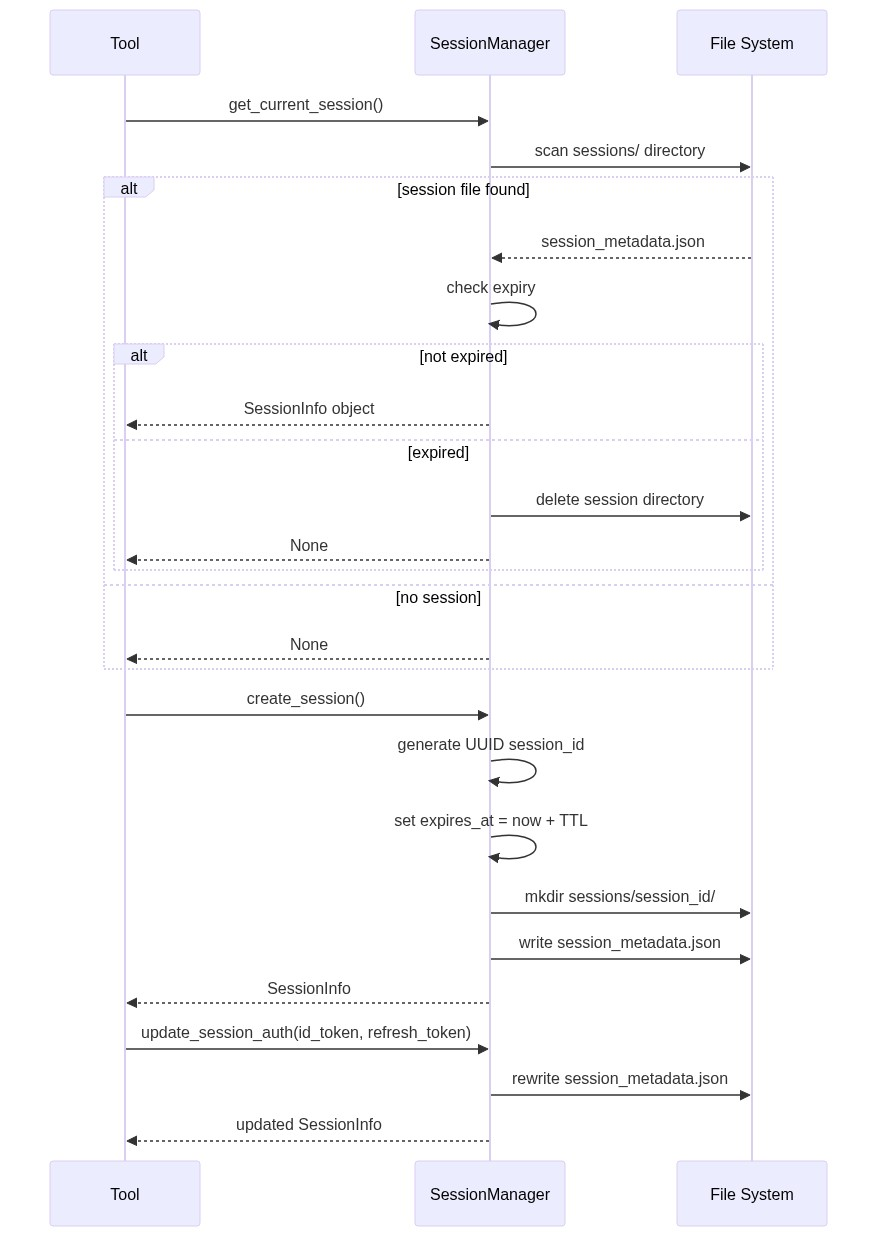
\includegraphics[width=\linewidth]{03_session_lifecycle.png}
  \caption{Session creation, loading, and expiry sequence}
  \label{fig:session}
\end{figure}

\subsection{Key Methods}

\begin{center}
\begin{tabularx}{\linewidth}{lX}
  \toprule
  \textbf{Method} & \textbf{Description} \\
  \midrule
  \texttt{create\_session()} & Generates UUID, sets expiry from \texttt{SESSION\_TTL\_HOURS}, writes metadata to disk \\
  \texttt{get\_current\_session()} & Scans disk for existing non-expired session; returns \texttt{None} if none found \\
  \texttt{load\_session(path)} & Reads \texttt{session\_metadata.json}; deletes directory if expired \\
  \texttt{update\_session\_auth(tokens)} & Writes JWT tokens + expiry back to the metadata file \\
  \texttt{get\_valid\_id\_token()} & Returns current token if valid; otherwise calls the refresh endpoint automatically \\
  \texttt{cleanup\_session(session\_id)} & Removes session directory from disk \\
  \bottomrule
\end{tabularx}
\end{center}

\section{\texttt{core/handle\_manager.py} --- Data Storage}

\begin{mdframed}[style=filebox]
\textbf{File:} \texttt{core/handle\_manager.py} \quad
\textbf{Class:} \texttt{HandleManager}
\end{mdframed}

\subsection{Responsibility}

Provides a simple \emph{handle-based} key-value store backed by JSON files.
A handle is just a filename --- tools store large API responses and get back
a compact handle string they can pass to other tools.

\subsection{Handle Format}

\begin{lstlisting}[language={},caption={Handle filename format}]
{data_type}_{location}_{YYYYMMDDHHMMSSF}_{uuid8}.json
# Example:
geospatial_data_riyadh_20260418_213401_123456_a1b2c3d4.json
\end{lstlisting}

The microsecond component (\texttt{\%f}) ensures uniqueness even for
back-to-back calls within the same second.

\subsection{Data Flow}

\begin{figure}[H]
  \centering
  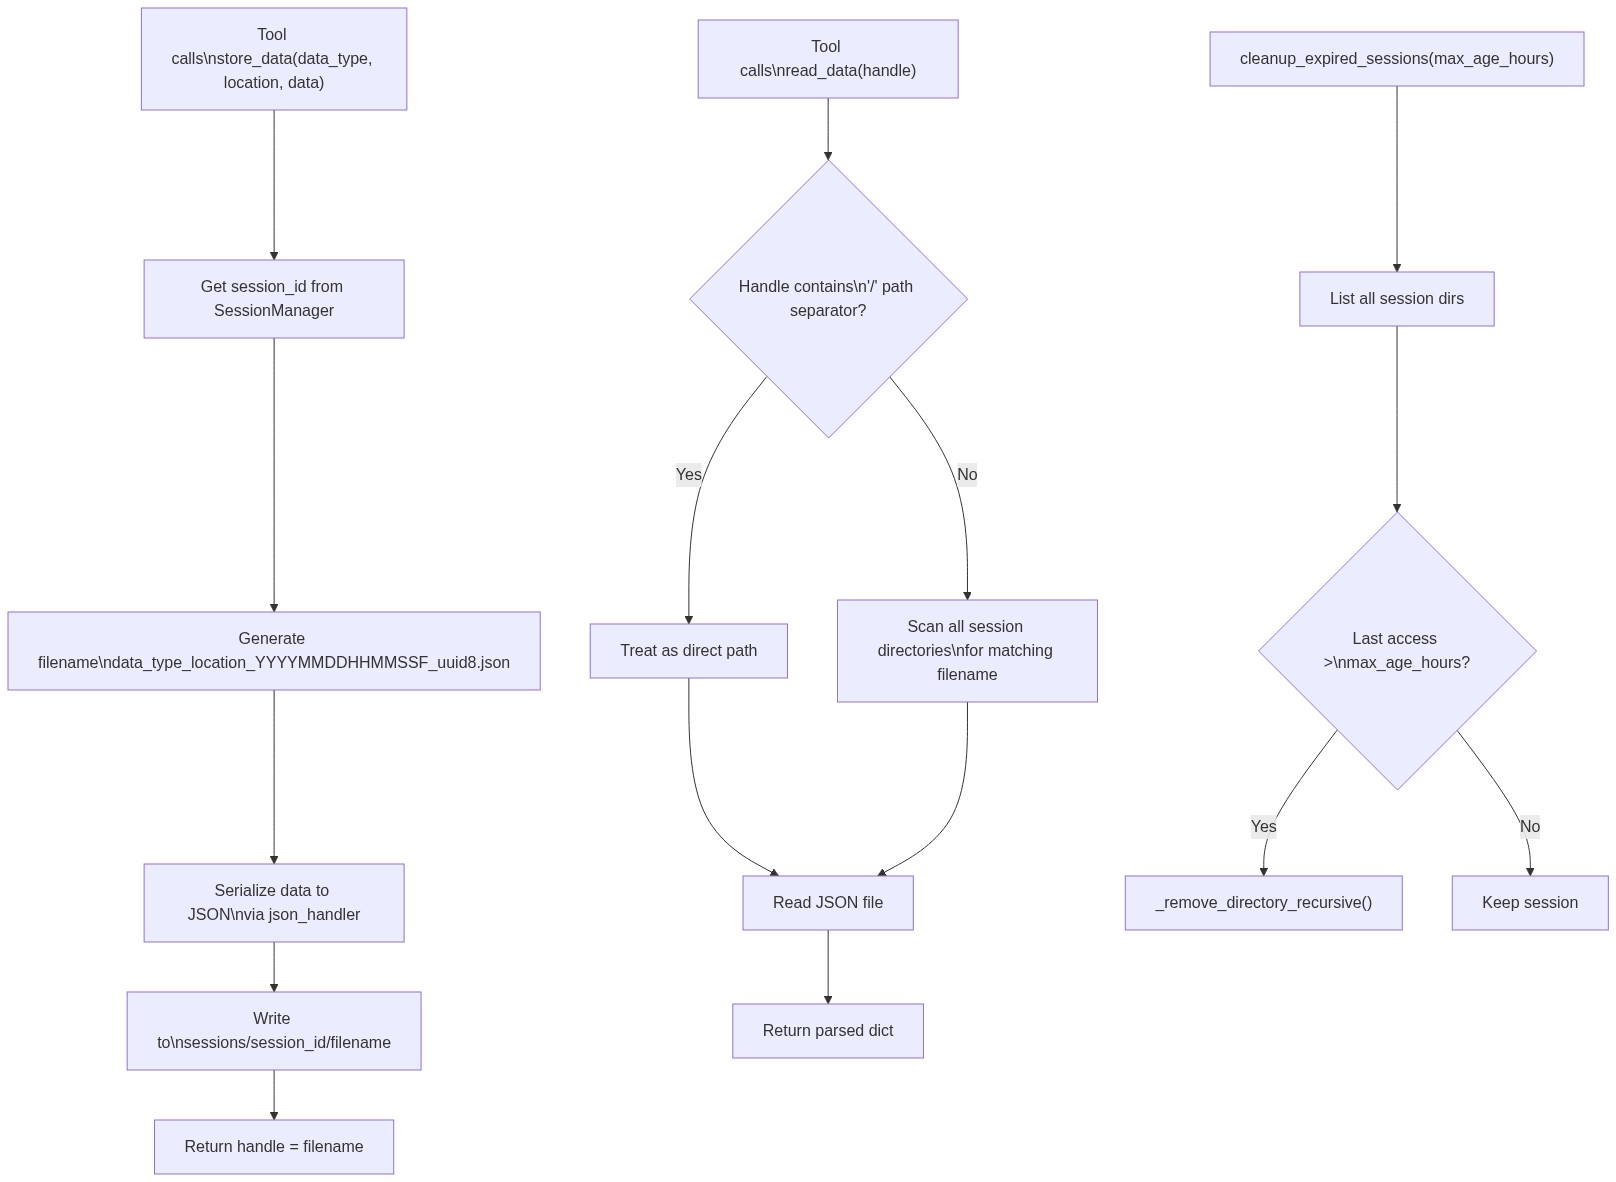
\includegraphics[width=\linewidth]{05_handle_manager_flow.png}
  \caption{HandleManager store and retrieve flow}
  \label{fig:handle}
\end{figure}

\subsection{Cleanup Methods}

\begin{center}
\begin{tabularx}{\linewidth}{lX}
  \toprule
  \textbf{Method} & \textbf{Trigger Condition} \\
  \midrule
  \texttt{cleanup\_expired\_sessions(max\_age\_hours)} & Sessions older than TTL \\
  \texttt{cleanup\_large\_sessions(max\_size\_mb)} & Sessions exceeding 100 MB \\
  \texttt{cleanup\_oldest\_sessions(keep\_n)} & Total storage $>$ 500 MB \\
  \texttt{get\_storage\_stats()} & Returns per-session and total size metrics \\
  \bottomrule
\end{tabularx}
\end{center}

\section{\texttt{core/cleanup.py} --- Background Cleanup Task}

\begin{mdframed}[style=filebox]
\textbf{File:} \texttt{core/cleanup.py}
\end{mdframed}

An infinite \texttt{async} coroutine that runs in the background throughout the
server's lifetime. It enforces three storage policies in sequence on every tick:

\begin{figure}[H]
  \centering
  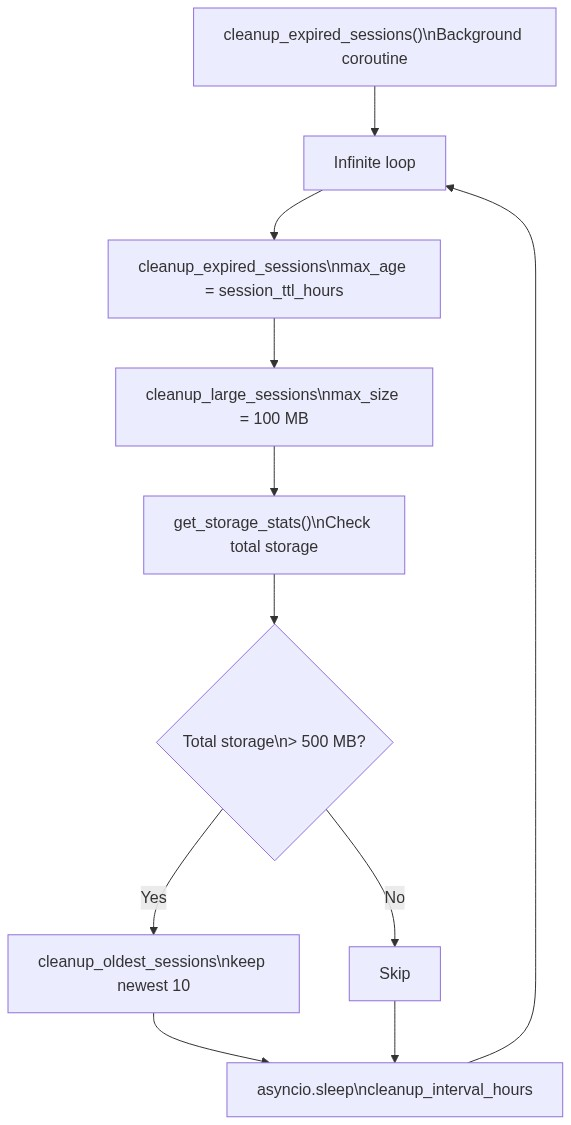
\includegraphics[width=0.75\linewidth]{11_cleanup_flow.png}
  \caption{Background cleanup loop}
  \label{fig:cleanup}
\end{figure}

% ============================================================
\chapter{Utility Modules}
% ============================================================

\section{\texttt{utils/json\_handler.py} --- Async JSON I/O}

\begin{mdframed}[style=filebox]
\textbf{File:} \texttt{utils/json\_handler.py}
\end{mdframed}

Handles reading and writing JSON files safely in an async context:

\begin{itemize}[noitemsep]
  \item \textbf{\texttt{FileLock}} --- simple async lock that prevents two coroutines from
    writing the same file simultaneously (avoids corruption)
  \item \textbf{\texttt{to\_serializable()}} --- recursively converts Pydantic models,
    \texttt{datetime} objects, sets, etc.\ to plain Python types before JSON serialisation
  \item \textbf{\texttt{use\_json(path, mode, data)}} --- async read (\texttt{'r'}) or write (\texttt{'w'})
    with automatic file locking; used by both managers
\end{itemize}

\section{\texttt{utils/http\_client.py} --- Backend HTTP Client}

\begin{mdframed}[style=filebox]
\textbf{File:} \texttt{utils/http\_client.py}
\end{mdframed}

All communication with the backend REST API goes through two functions here:

\begin{figure}[H]
  \centering
  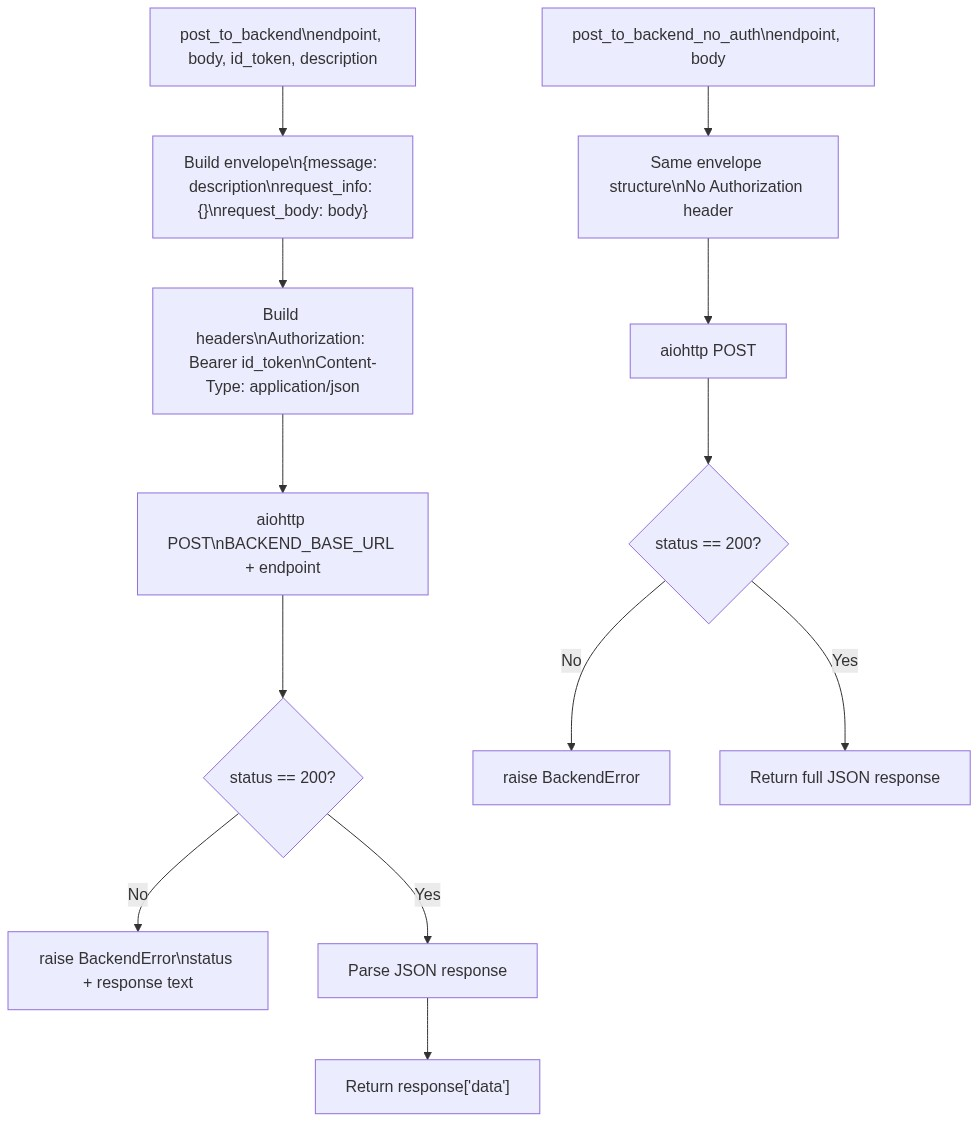
\includegraphics[width=\linewidth]{12_http_client_flow.png}
  \caption{HTTP client request envelope and error handling}
  \label{fig:http}
\end{figure}

Every request wraps the payload in a standard envelope:
\begin{lstlisting}[language=Python, caption={Request envelope structure}]
{
    "message":      description,   # human-readable description for the backend log
    "request_info": {},            # reserved for future metadata
    "request_body": body           # actual payload (dict from Pydantic .model_dump())
}
\end{lstlisting}

\textbf{\texttt{BackendError}} is raised for any non-200 response and carries
the HTTP status code and raw response text so tool functions can surface
a helpful error message to the AI client.

\section{\texttt{utils/auth\_helpers.py} --- Centralised Auth Check}

\begin{mdframed}[style=filebox]
\textbf{File:} \texttt{utils/auth\_helpers.py}
\end{mdframed}

\texttt{require\_auth(session\_manager)} is called at the top of \emph{every}
tool function that needs an authenticated user. It:

\begin{enumerate}[noitemsep]
  \item Calls \texttt{session\_manager.get\_current\_session()}
  \item If no session exists, creates a new one
  \item Checks that the session has a valid \texttt{id\_token}
  \item Calls \texttt{get\_valid\_id\_token()} which refreshes the token if expired
  \item Returns \texttt{(session, user\_id, id\_token)} on success, or an error string
\end{enumerate}

Returning a plain error string (instead of raising an exception) means the
MCP tool can pass it back to the AI client as a readable message.

% ============================================================
\chapter{MCP Server Entry Point}
% ============================================================

\section{\texttt{mcp\_server.py} --- Server Bootstrap}

\begin{mdframed}[style=filebox]
\textbf{File:} \texttt{mcp\_server.py} \quad \textbf{Entry point:} \texttt{python mcp\_server.py}
\end{mdframed}

\subsection{Startup Sequence}

When you run \texttt{python mcp\_server.py}, the following happens in order:

\begin{enumerate}[noitemsep]
  \item \textbf{Module imports} --- all tools, core managers, and config loaded
  \item \textbf{Global singletons created} --- \texttt{SessionManager()} then \texttt{HandleManager(session\_manager)}
  \item \textbf{\texttt{FastMCPWithCORS} instantiated} --- server named \texttt{"saudi-location-intelligence"}
  \item \textbf{All tools registered} --- seven \texttt{register\_*(mcp)} calls
  \item \textbf{\texttt{main()} called} --- logs startup info, calls \texttt{mcp.run("sse")}
  \item \textbf{Uvicorn started} --- listens on \texttt{SERVER\_HOST:SERVER\_PORT}
\end{enumerate}

\subsection{FastMCPWithCORS}

This subclass of \texttt{FastMCP} adds two overrides:

\begin{center}
\begin{tabularx}{\linewidth}{lX}
  \toprule
  \textbf{Override} & \textbf{Why} \\
  \midrule
  \texttt{sse\_app()} & Wraps the Starlette app with \texttt{CORSMiddleware} so browser-based clients (MCP Inspector) can connect \\
  \texttt{run()} & Forces the bind address to \texttt{SERVER\_HOST} (default \texttt{0.0.0.0}) instead of \texttt{127.0.0.1}, which is required for Docker \\
  \bottomrule
\end{tabularx}
\end{center}

\subsection{MCP Resources}

Two read-only \emph{resources} are registered (queryable by MCP clients):

\begin{center}
\begin{tabularx}{\linewidth}{lX}
  \toprule
  \textbf{URI} & \textbf{Returns} \\
  \midrule
  \texttt{session://current} & Current session ID and expiry timestamp (or ``No active session'') \\
  \texttt{config://server} & Server configuration summary: TTL, storage path, available tools \\
  \bottomrule
\end{tabularx}
\end{center}

\subsection{Expected Terminal Output}

\begin{lstlisting}[language={},caption={Terminal output on startup}]
INFO  mcp_server - [wrench] Main logging initialized
INFO  mcp_server - [SA] Saudi Location Intelligence MCP Server
INFO  mcp_server - Starting SSE transport on http://0.0.0.0:8001/sse
INFO  mcp_server - Connect MCP Inspector to: http://localhost:8001/sse
INFO  uvicorn - Started server process [PID]
INFO  uvicorn - Uvicorn running on http://0.0.0.0:8001
\end{lstlisting}

% ============================================================
\chapter{Tool Modules}
% ============================================================

\section{Generic Tool Execution Flow}

All tools follow the same pattern. Figure~\ref{fig:tool} shows the complete
sequence from AI client call to response.

\begin{figure}[H]
  \centering
  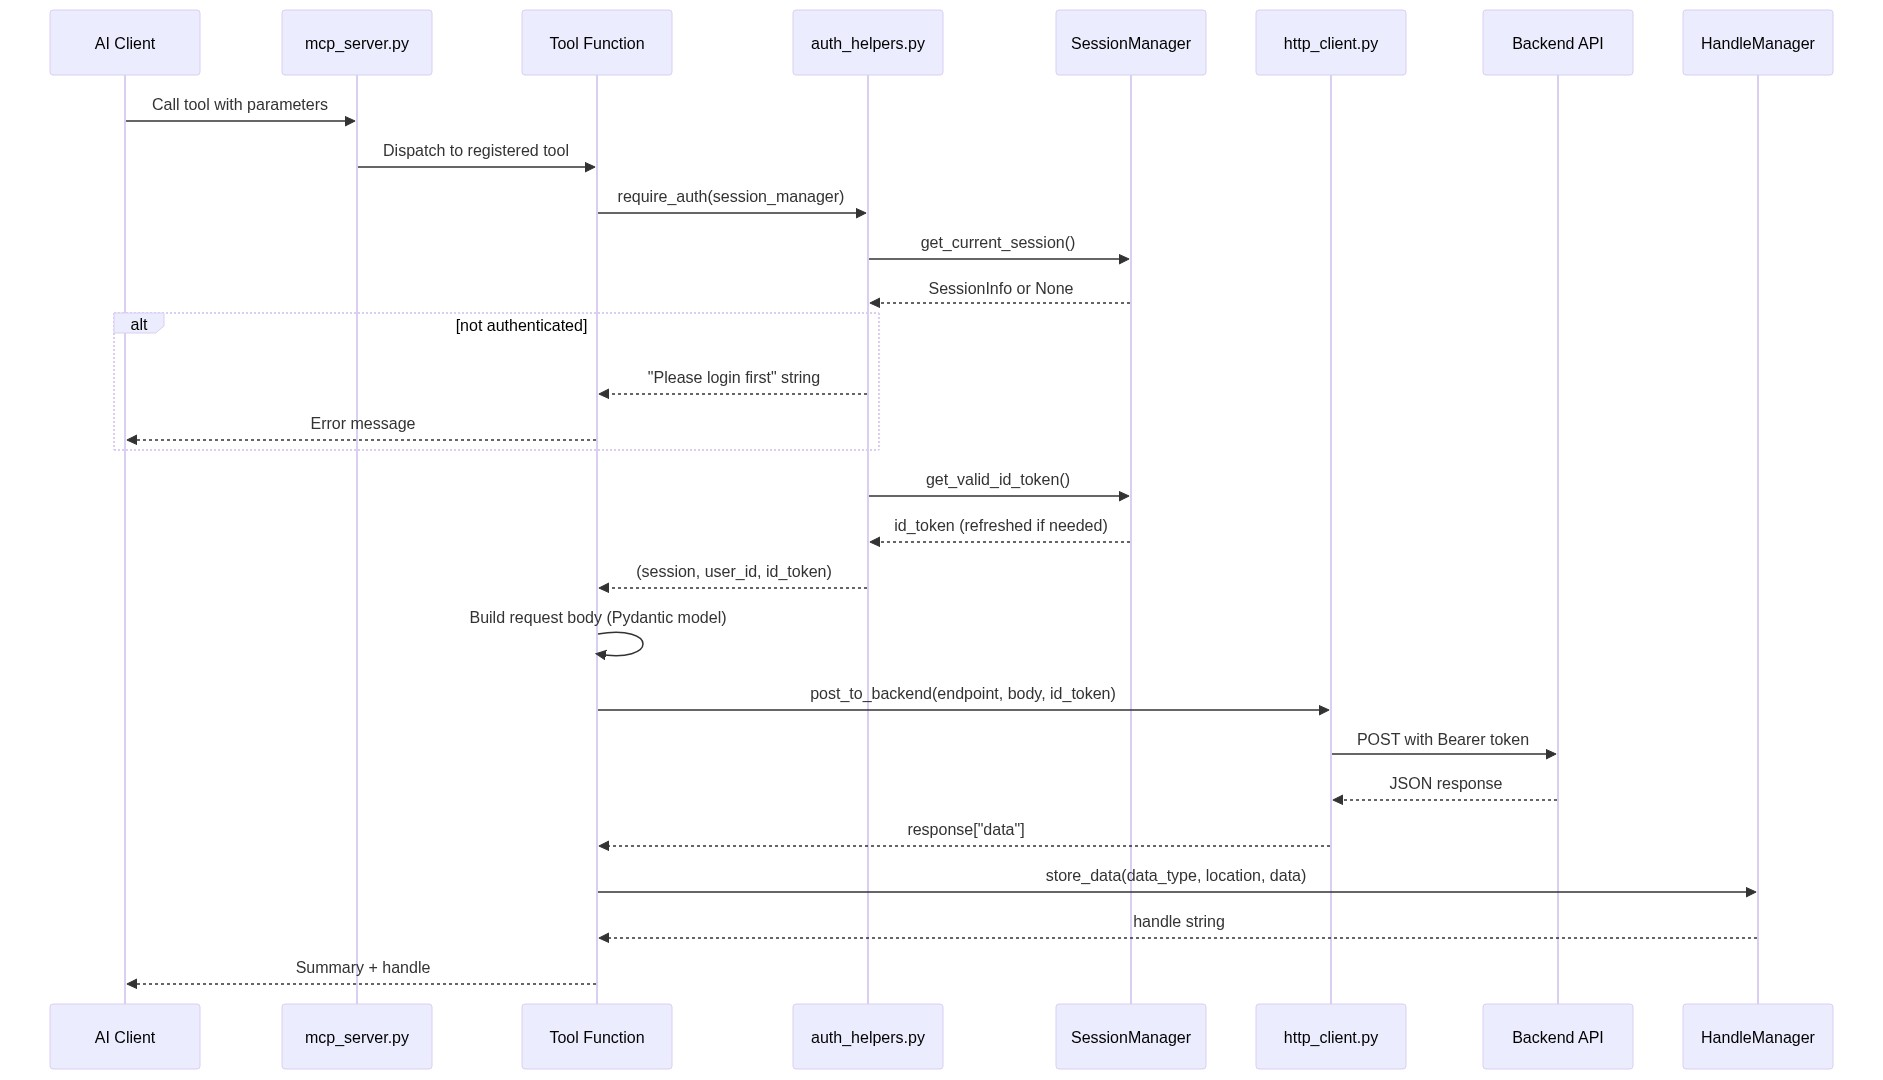
\includegraphics[width=\linewidth]{06_tool_execution_flow.png}
  \caption{Generic tool execution sequence}
  \label{fig:tool}
\end{figure}

\section{\texttt{tools/auth\_tools.py} --- Authentication Tools}

\begin{mdframed}[style=filebox]
\textbf{File:} \texttt{tools/auth\_tools.py} \quad \textbf{Registers:} 4 tools
\end{mdframed}

\subsection{Authentication Flow}

\begin{figure}[H]
  \centering
  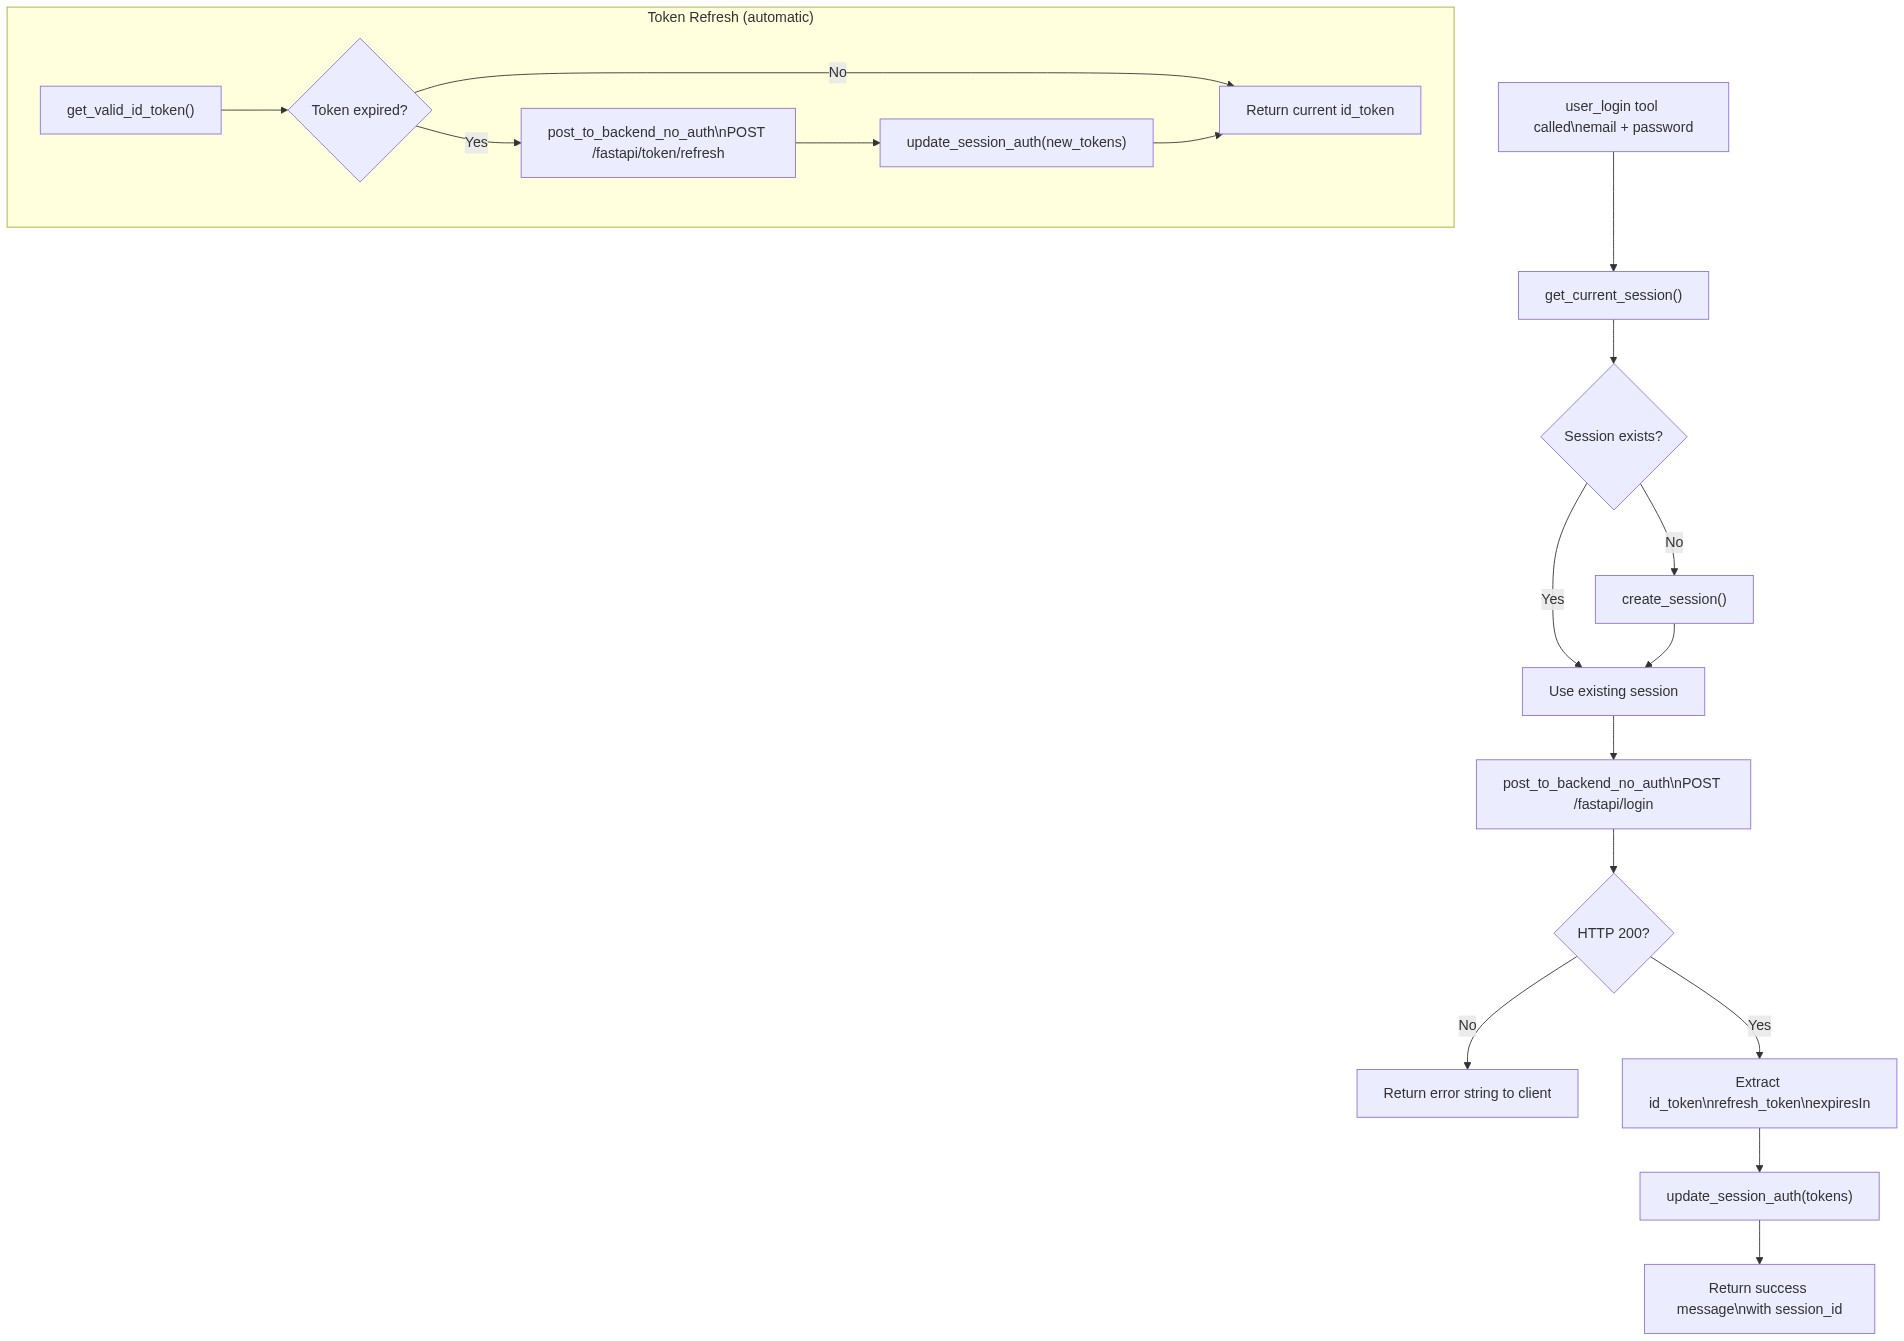
\includegraphics[width=0.9\linewidth]{04_auth_flow.png}
  \caption{user\_login authentication flow}
  \label{fig:auth}
\end{figure}

\subsection{Registered Tools}

\begin{center}
\begin{tabularx}{\linewidth}{lX}
  \toprule
  \textbf{Tool name} & \textbf{Description} \\
  \midrule
  \texttt{user\_login} & Authenticates with email + password; stores JWT tokens in session \\
  \texttt{list\_stored\_data} & Lists all data files currently stored in the session directory \\
  \texttt{get\_data\_from\_handle} & Reads a stored JSON file by handle and returns its content \\
  \texttt{get\_current\_session\_logs} & Returns the last N lines of the session log file \\
  \bottomrule
\end{tabularx}
\end{center}

\section{\texttt{tools/geospatial.py} --- Geospatial Data Fetcher}

\begin{mdframed}[style=filebox]
\textbf{File:} \texttt{tools/geospatial.py} \quad \textbf{Registers:} 1 tool
\end{mdframed}

\subsection{Tool: \texttt{fetch\_geospatial\_data}}

Fetches GeoJSON data from the backend for a given Saudi city and search query.
The full dataset is stored server-side; only a handle + summary is returned.

\begin{figure}[H]
  \centering
  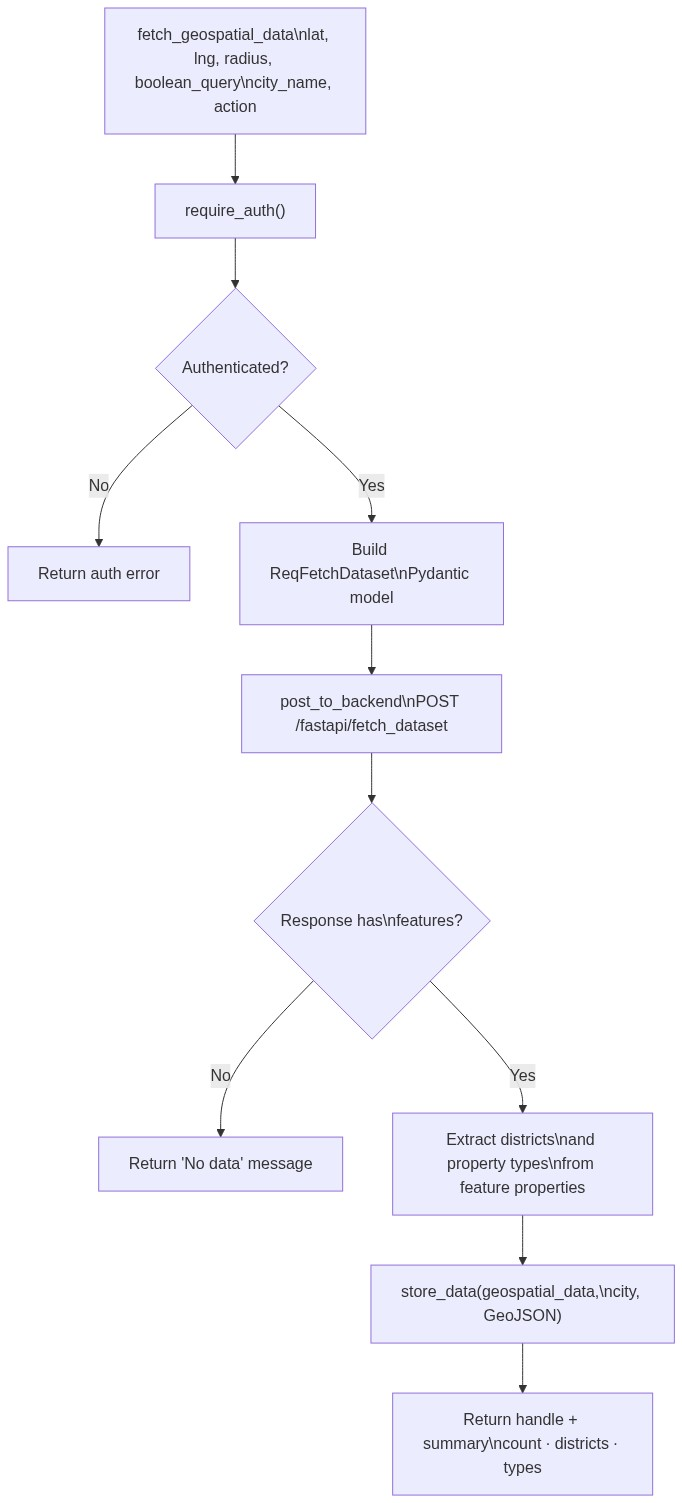
\includegraphics[width=0.85\linewidth]{07_geospatial_flow.png}
  \caption{fetch\_geospatial\_data flow}
  \label{fig:geo}
\end{figure}

\subsubsection{Parameters}

\begin{center}
\begin{tabularx}{\linewidth}{llX}
  \toprule
  \textbf{Parameter} & \textbf{Default} & \textbf{Description} \\
  \midrule
  \texttt{lat}, \texttt{lng} & required & Search centre coordinates \\
  \texttt{radius} & 5000 m & Search radius in metres \\
  \texttt{boolean\_query} & required & e.g.\ \texttt{"restaurant AND NOT fast\_food"} \\
  \texttt{city\_name} & required & Saudi city (Riyadh, Jeddah, etc.) \\
  \texttt{action} & \texttt{"sample"} & \texttt{"sample"} (20 records) or \texttt{"full data"} \\
  \texttt{include\_rating\_info} & \texttt{False} & Include review/rating data \\
  \texttt{include\_only\_sub\_properties} & \texttt{True} & Return compact property set \\
  \bottomrule
\end{tabularx}
\end{center}

\subsubsection{Return Value}

\begin{lstlisting}[language={},caption={Example return value}]
OK  Data fetched. Handle: `geospatial_data_riyadh_20260418_214501_123456_a1b2c3d4.json`.
Summary: 47 records found for 'warehouse OR logistics' in Riyadh.
Districts: ['Al Malaz', 'Al Quds', 'Al Salam'].
Types: ['warehouse', 'logistics_center'].
\end{lstlisting}

\section{\texttt{tools/optimize\_sales\_territories.py} --- Territory Optimisation}

\begin{mdframed}[style=filebox]
\textbf{File:} \texttt{tools/optimize\_sales\_territories.py} \quad \textbf{Registers:} 1 tool
\end{mdframed}

\subsection{Tool: \texttt{optimize\_sales\_territories}}

Uses spatial clustering on the backend to divide a city's business locations
into balanced sales territories. Metrics returned include:

\begin{itemize}[noitemsep]
  \item Market equity score (Coefficient of Variation across territories)
  \item Population distribution per territory
  \item Accessibility analysis (drive-time coverage)
  \item Service gap identification
\end{itemize}

\subsubsection{Key Parameters}

\begin{center}
\begin{tabularx}{\linewidth}{llX}
  \toprule
  \textbf{Parameter} & \textbf{Default} & \textbf{Description} \\
  \midrule
  \texttt{city\_name} & required & Target Saudi city \\
  \texttt{num\_sales\_man} & required & Number of sales representatives / territories \\
  \texttt{distance\_limit} & 2.5 km & Maximum intra-territory distance \\
  \texttt{boolean\_query} & required & Business type to cluster \\
  \texttt{include\_raw\_data} & \texttt{False} & Include raw clustering data in handle \\
  \bottomrule
\end{tabularx}
\end{center}

% ============================================================
\chapter{Analysis Tools}
% ============================================================

\section{\texttt{tools/analysis\_tools/hub\_analyzer.py} --- Hub Expansion Analysis}

\begin{mdframed}[style=filebox]
\textbf{File:} \texttt{tools/analysis\_tools/hub\_analyzer.py} \quad \textbf{Registers:} 1 tool
\end{mdframed}

\subsection{Tool: \texttt{hub\_expansion\_analyzer}}

Scores potential hub locations using five weighted criteria:

\begin{enumerate}[noitemsep]
  \item Target proximity --- distance to key demand points
  \item Population access --- how many people can reach the hub
  \item Rent efficiency --- cost vs.\ footfall ratio
  \item Competitive advantage --- distance from competing hubs
  \item Population coverage --- broader catchment area
\end{enumerate}

\begin{figure}[H]
  \centering
  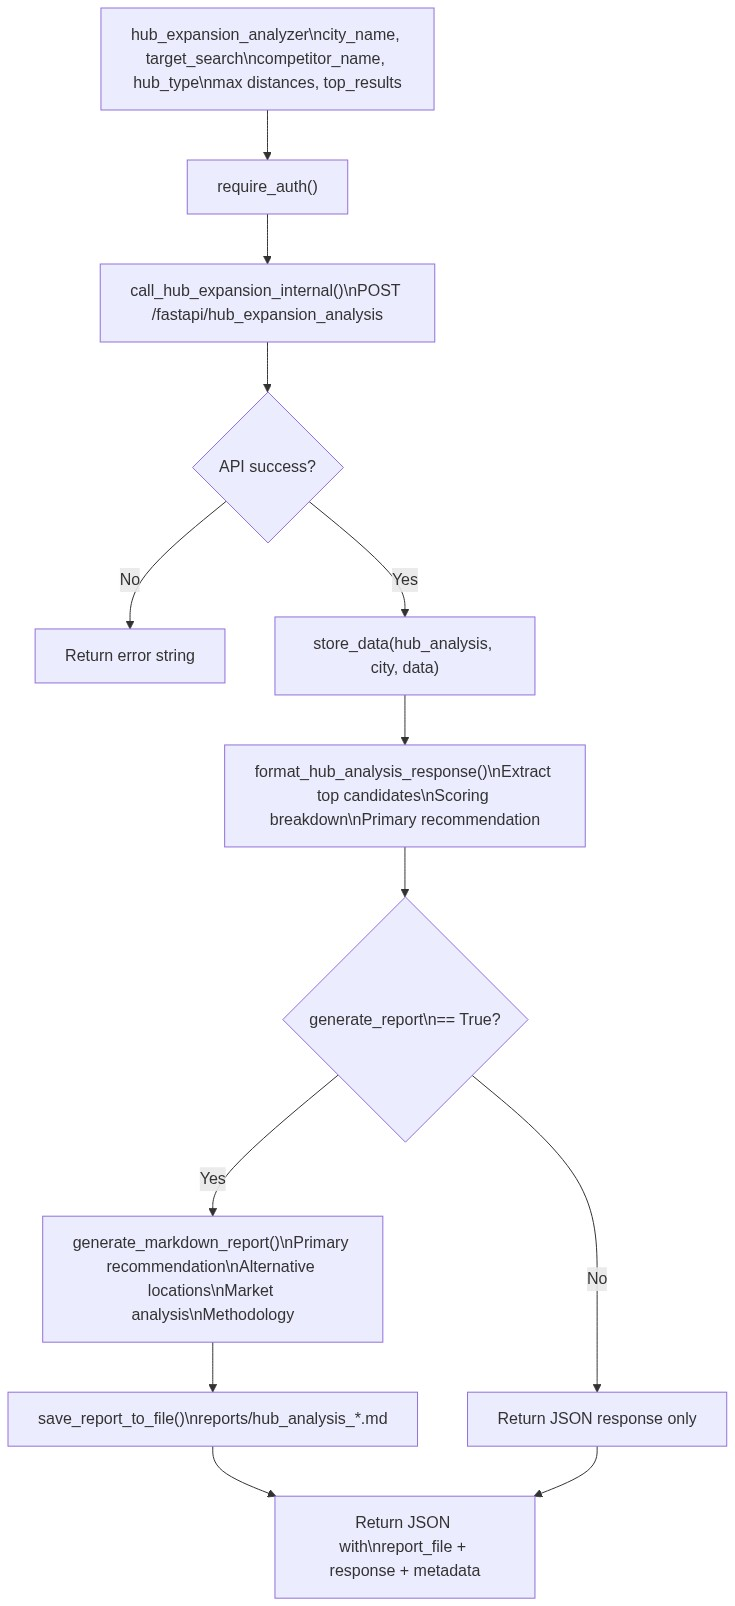
\includegraphics[width=\linewidth]{08_hub_analyzer_flow.png}
  \caption{hub\_expansion\_analyzer flow with optional report generation}
  \label{fig:hub}
\end{figure}

\subsubsection{Report Generation}

When \texttt{generate\_report=True}, the tool creates a Markdown file in
\texttt{reports/} containing:
\begin{itemize}[noitemsep]
  \item Primary recommendation with full scoring breakdown
  \item Alternative candidate locations
  \item Market analysis and competitor mapping
  \item Methodology explanation
\end{itemize}

\section{\texttt{tools/analysis\_tools/pharmacy\_analyzer.py} --- Pharmacy Site Selection}

\begin{mdframed}[style=filebox]
\textbf{File:} \texttt{tools/analysis\_tools/pharmacy\_analyzer.py} \quad \textbf{Registers:} 1 tool
\end{mdframed}

\subsection{Tool: \texttt{generate\_pharmacy\_report}}

Scores pharmacy locations using five configurable weight factors:

\begin{figure}[H]
  \centering
  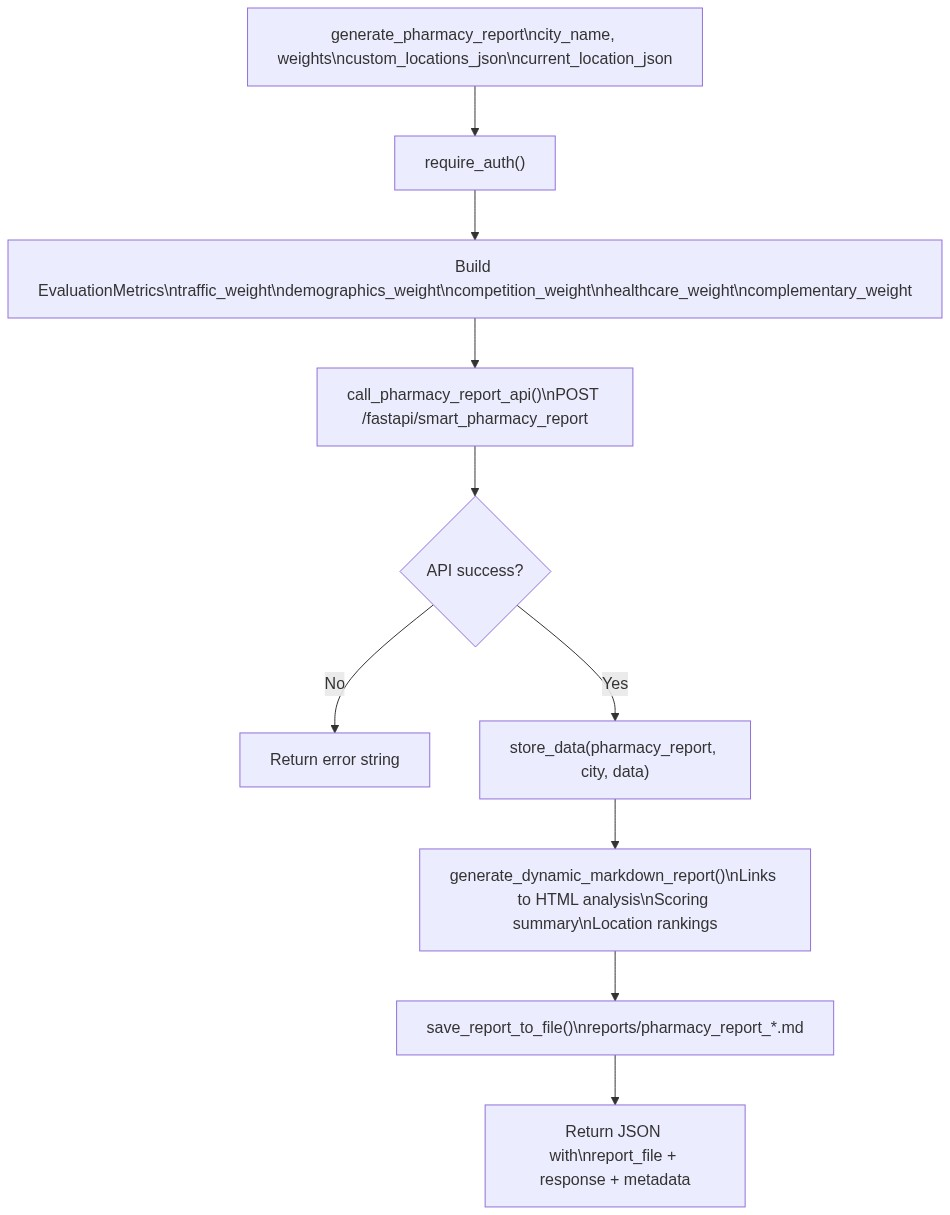
\includegraphics[width=0.9\linewidth]{09_pharmacy_flow.png}
  \caption{generate\_pharmacy\_report flow}
  \label{fig:pharmacy}
\end{figure}

\subsubsection{Scoring Weights (all default to equal)}

\begin{center}
\begin{tabularx}{\linewidth}{lX}
  \toprule
  \textbf{Weight Parameter} & \textbf{What it measures} \\
  \midrule
  \texttt{traffic\_weight}        & Foot traffic and vehicular accessibility \\
  \texttt{demographics\_weight}   & Population density and age distribution \\
  \texttt{competition\_weight}    & Proximity to competing pharmacies \\
  \texttt{healthcare\_weight}     & Nearby hospitals, clinics, medical centres \\
  \texttt{complementary\_weight}  & Co-located complementary businesses (supermarkets, etc.) \\
  \bottomrule
\end{tabularx}
\end{center}

Custom locations can be passed as a JSON string (\texttt{custom\_locations\_json})
to evaluate specific addresses instead of the backend's suggestions.

% ============================================================
\chapter{Report Tools}
% ============================================================

\section{\texttt{tools/report\_tools/generate\_report.py} --- Report Generation}

\begin{mdframed}[style=filebox]
\textbf{File:} \texttt{tools/report\_tools/generate\_report.py} \quad \textbf{Registers:} 1 tool
\end{mdframed}

\subsection{Tool: \texttt{generate\_territory\_report}}

Takes a \texttt{data\_handle} (from \texttt{optimize\_sales\_territories}) and produces
a formatted Markdown report. Three report types are available:

\begin{figure}[H]
  \centering
  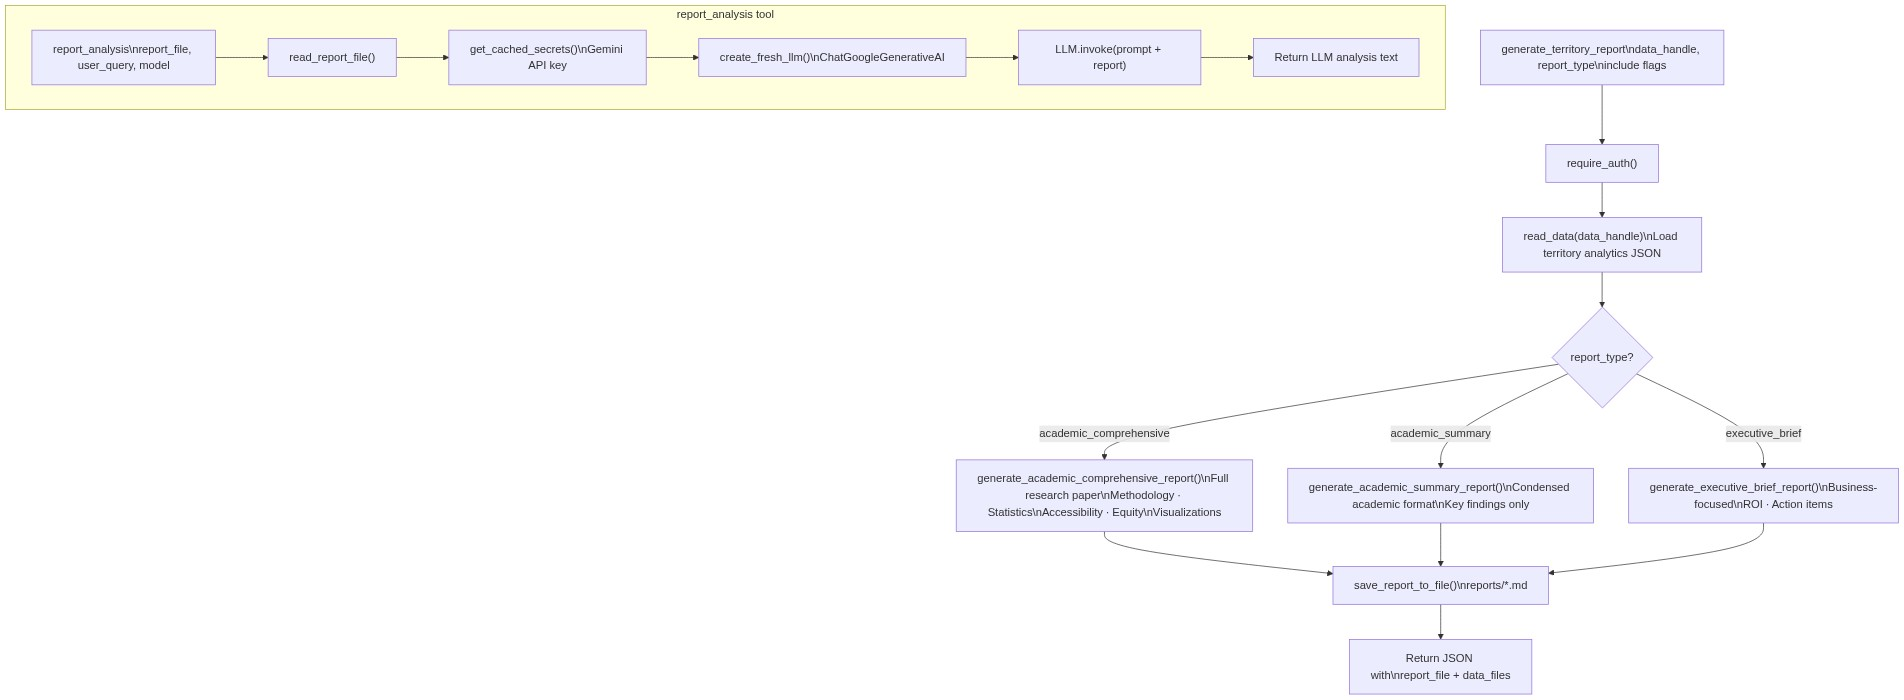
\includegraphics[width=\linewidth]{10_report_generation_flow.png}
  \caption{Report generation and LLM analysis flow}
  \label{fig:report}
\end{figure}

\begin{center}
\begin{tabularx}{\linewidth}{lX}
  \toprule
  \textbf{Report Type} & \textbf{Contents} \\
  \midrule
  \texttt{academic\_comprehensive} & Full research paper: methodology, statistics, accessibility, equity analysis, bibliography \\
  \texttt{academic\_summary}       & Condensed academic format; key findings and tables only \\
  \texttt{executive\_brief}        & Business-focused: ROI, action items, risk summary \\
  \bottomrule
\end{tabularx}
\end{center}

\subsubsection{Statistical Analysis Functions}

The report generator includes several helper functions that derive statistics
from raw territory data:

\begin{itemize}[noitemsep]
  \item \texttt{extract\_territory\_metrics()} --- mean, std, CV, min, max per metric
  \item \texttt{assess\_balance\_quality(cv)} --- classifies balance as Excellent/Good/Moderate/Poor
  \item \texttt{generate\_equity\_analysis()} --- validates whether territory sizes are balanced
  \item \texttt{generate\_accessibility\_analysis()} --- service coverage within drive-time bands
\end{itemize}

\section{\texttt{tools/report\_tools/report\_analysis.py} --- LLM Report Analysis}

\begin{mdframed}[style=filebox]
\textbf{File:} \texttt{tools/report\_tools/report\_analysis.py} \quad \textbf{Registers:} 1 tool
\end{mdframed}

\subsection{Tool: \texttt{report\_analysis}}

Reads a saved Markdown report from disk and sends it to a Google Gemini LLM
along with the user's query. Returns a natural language answer.

\subsubsection{Implementation Details}

\begin{itemize}[noitemsep]
  \item Uses \textbf{LangChain} (\texttt{ChatGoogleGenerativeAI}) as the LLM abstraction
  \item Default model: \texttt{gemini-2.5-flash}
  \item API key loaded from \texttt{secrets/secrets\_llm.json} (cached after first load)
  \item A fresh LLM instance is created per call to avoid event-loop conflicts
  \item Unicode characters in reports are sanitised before sending to avoid encoding issues
\end{itemize}

% ============================================================
\chapter{End-to-End Data Flows}
% ============================================================

\section{Complete Geospatial Analysis Workflow}

A typical end-to-end usage from the AI client perspective:

\begin{enumerate}
  \item \textbf{Login} --- Call \texttt{user\_login} with email + password.
    Session created, JWT stored.
  \item \textbf{Fetch data} --- Call \texttt{fetch\_geospatial\_data} with lat/lng
    and a boolean query. Receive a handle like
    \texttt{geospatial\_data\_riyadh\_*.json}.
  \item \textbf{Optimise territories} --- Call \texttt{optimize\_sales\_territories}
    with \texttt{city\_name}, \texttt{num\_sales\_man}, same query. Receive a
    territory analytics handle.
  \item \textbf{Generate report} --- Call \texttt{generate\_territory\_report} with
    the territory handle. Receive a Markdown report file path.
  \item \textbf{Analyse report} --- Call \texttt{report\_analysis} with the report
    file path and a natural language question. Receive Gemini's answer.
\end{enumerate}

\section{Token Refresh Cycle}

JWT ID tokens expire after \texttt{expiresIn} seconds (returned by the login
endpoint). \texttt{get\_valid\_id\_token()} checks expiry before every tool call
and automatically calls \texttt{/fastapi/token/refresh} if needed. This is
transparent to the AI client --- it never needs to call \texttt{user\_login} again
within a session.

% ============================================================
\chapter{Deployment}
% ============================================================

\section{Running Locally}

\begin{lstlisting}[language={},caption={Local startup}]
# Install dependencies
uv sync

# Start server
python mcp_server.py
# or
uv run slocator-mcp

# Connect MCP Inspector to:
# http://localhost:8001/sse
\end{lstlisting}

\section{Running with Docker}

\begin{lstlisting}[language={},caption={Docker build and run}]
docker build -t slocator-mcp .

docker run -p 8001:8001 \
  -e BACKEND_URL=http://your-backend:8000 \
  -e MCP_SERVER_PORT=8001 \
  -e SESSION_TTL_HOURS=8 \
  slocator-mcp
\end{lstlisting}

\subsection{Dockerfile Highlights}

\begin{itemize}[noitemsep]
  \item Base image: \texttt{python:3.13-slim}
  \item Package manager: \texttt{uv} (fast, no pip)
  \item Non-root user: \texttt{appuser} (UID 1000) for security
  \item Health check: HTTP GET to \texttt{/sse} endpoint on port 8001
  \item Runtime directories (\texttt{sessions/}, \texttt{reports/}, \texttt{logs/})
    created at build time with correct ownership
\end{itemize}

\section{Environment Variables Reference}

\begin{center}
\begin{tabularx}{\linewidth}{llX}
  \toprule
  \textbf{Variable} & \textbf{Default} & \textbf{Description} \\
  \midrule
  \texttt{BACKEND\_URL}            & \texttt{http://localhost:8000} & Backend REST API base URL \\
  \texttt{MCP\_HOST}               & \texttt{0.0.0.0}              & Bind address \\
  \texttt{MCP\_SERVER\_PORT}       & \texttt{8001}                 & Port \\
  \texttt{CORS\_ORIGINS}           & \texttt{*}                    & Comma-separated CORS origins \\
  \texttt{SESSION\_TTL\_HOURS}     & \texttt{8}                    & Session lifetime \\
  \texttt{CLEANUP\_INTERVAL\_HOURS} & \texttt{1}                   & Cleanup loop interval \\
  \bottomrule
\end{tabularx}
\end{center}

% ============================================================
\chapter{Project File Index}
% ============================================================

\begin{center}
\begin{longtable}{lp{9cm}}
  \toprule
  \textbf{File} & \textbf{Purpose} \\
  \midrule
  \endfirsthead
  \toprule
  \textbf{File} & \textbf{Purpose} \\
  \midrule
  \endhead
  \texttt{mcp\_server.py}                              & Entry point; server bootstrap and tool registration \\
  \texttt{config.py}                                   & Configuration loader with env-var overrides \\
  \texttt{config.json}                                 & Default runtime configuration \\
  \texttt{logging\_config.py}                          & Structured logging setup \\
  \texttt{models.py}                                   & \texttt{DataHandle} and \texttt{SessionInfo} Pydantic models \\
  \texttt{context.py}                                  & \texttt{AppContext} dataclass and lazy-import helper \\
  \texttt{core/session\_manager.py}                    & Session lifecycle, JWT storage, token refresh \\
  \texttt{core/handle\_manager.py}                     & File-backed key-value store; cleanup policies \\
  \texttt{core/cleanup.py}                             & Infinite async cleanup coroutine \\
  \texttt{utils/json\_handler.py}                      & Async JSON file I/O with file locking \\
  \texttt{utils/http\_client.py}                       & Backend HTTP client; \texttt{BackendError} \\
  \texttt{utils/auth\_helpers.py}                      & \texttt{require\_auth()} guard used by all tools \\
  \texttt{all\_types/request\_dtypes.py}               & Pydantic request models for backend API \\
  \texttt{tools/auth\_tools.py}                        & login, list data, read handle, session logs \\
  \texttt{tools/geospatial.py}                         & \texttt{fetch\_geospatial\_data} tool \\
  \texttt{tools/optimize\_sales\_territories.py}       & \texttt{optimize\_sales\_territories} tool \\
  \texttt{tools/analysis\_tools/hub\_analyzer.py}      & \texttt{hub\_expansion\_analyzer} tool \\
  \texttt{tools/analysis\_tools/pharmacy\_analyzer.py} & \texttt{generate\_pharmacy\_report} tool \\
  \texttt{tools/report\_tools/generate\_report.py}     & \texttt{generate\_territory\_report} tool \\
  \texttt{tools/report\_tools/report\_analysis.py}     & \texttt{report\_analysis} LLM tool \\
  \texttt{pyproject.toml}                              & Project metadata and dependencies \\
  \texttt{Dockerfile}                                  & Container build definition \\
  \bottomrule
\end{longtable}
\end{center}

\end{document}